%Start with a Clear Heading: Begin your report with a heading that clearly states "Background" or "Introduction" to let readers know where to find this information.

%Provide an Overview: Begin by providing a brief overview of the project, including its title and purpose. You can mention what the project aims to achieve or the problem it intends to address.

%Contextualize the Project:

%Explain the broader context in which the project exists. Discuss any relevant industry trends, challenges, or issues that the project is responding to.
%Mention any external factors or events that have prompted the need for the project.
%If the project is part of a larger initiative or program, briefly introduce that program and explain how your project fits into it.
%Historical Background:

%Provide historical information if relevant. Explain how this project came into consideration, including any past efforts or developments leading up to it.
%If there are key milestones or events that are crucial to understanding the project's origins, mention them.
%State the Problem or Opportunity:

%Clearly state the problem or opportunity your project aims to address. Use data or facts to support your claims.
%If applicable, describe the significance of the problem or opportunity, such as its impact on the organization, stakeholders, or the community.
%Objective and Scope:

%Outline the specific objectives and scope of the project. What are you trying to achieve, and what are the boundaries or limitations of the project?
%Explain why these objectives are important and how they relate to solving the identified problem.
%Review of Relevant Literature:

%If there's existing research or literature relevant to your project, briefly mention it. This shows that you've conducted a literature review and are building upon prior knowledge.
%Highlight any gaps or areas where your project adds value or addresses shortcomings in existing research or practices.
%Cite Sources: Make sure to provide proper citations for any data, statistics, or information you use in this section.

%Keep it Concise and Engaging: While providing all necessary information, avoid making the background section overly long. Keep it engaging and focused on the most crucial information.

%Transition to the Next Sections: Conclude the background section by smoothly transitioning into the next sections of your report, such as the objectives, methodology, or project plan.

%Remember to tailor the background section to your specific project and audience. Your goal is to provide a comprehensive but concise overview that sets the stage for the reader to understand the significance and context of your project.

\chapter{Background}
\label{chap3}

\section{What are glitch attacks?}

Glitch attacks can be divided into two main categories: invasive (e.g., decapsulating the chip\cite{intro_to_hw_hacking}) and non-invasive attacks (e.g., electromagnetic fault injection (EMFI), voltage- and clock-glitching). Often times software and firmware security measures can only protect against non-invasive glitches, as protecting from invasive glitches often require hardware modifications\cite{glitchresistor}. Due to the nature of invasive attacks, it is beyond the scope of this project to defend against them. These often aim at tampering with Read-Only Memory (ROM) or Boot-loaders on Printed Circuit Boards (PCBs), and are not effective against more complex systems like a Central Processing Unit (CPU) or a System on Chip (SoC). 

Non-invasive glitches can be performed as long as an attacker has access to a device. However, there is quite a lot of procedural vulnerability discovery that has to be done before an attack can be performed. In the case of EMFI the chip has to be repeatedly exposed to electromagnetic interference during execution, to then determine which areas are most vulnerable to attacks\cite{emfi_injection}. An example of this being performed on the BCM2837 SoC can be seen in \autoref{fig:emfi_map}\cite{emfi_injection}. 

Voltage- or clock-glitching can be performed as long as there is some way to access these signals externally. Voltage-glitching often requires the removal of power filtering capacitors to gain more fine-grained control over a processor's voltage input. However, both of these methods require very precise timing by an attacker. This is why specialized tools such as the \textit{ChipWhisperer}\cite{chipWhisperer} are needed, as they allow extremely accurate fault-injection. These days it is also possible to perform effective glitch attacks with simple components in conjunction with a cheap Field Programmable Gate Array (FPGA) which outputs precise triggers\cite{hole_in_soc}. 

\begin{figure}[h!]
    \centering
    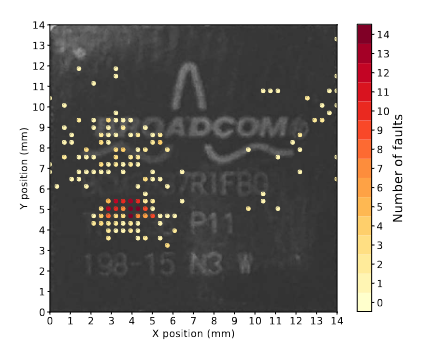
\includegraphics[scale=0.5]{docs/images/emfi_error_map.png}
    \caption{EMFI BCM2837 sensitivity map (dot size is not corralated with probe size.)\cite{emfi_injection}.}
    \label{fig:emfi_map}
\end{figure}

Voltage-glitching is performed by momentarily dropping the supply voltage during execution of critical operations. Clock-glitching is performed by altering clock timing to violate setup and hold time requirements of the hardware\cite{intro_to_FI}. The results of glitching cannot always be predicted, however they mainly result in skipped or repeated CPU instructions, incorrect evaluation of CPU instructions or corrupt reads from memory devices\cite{intro_to_FI}. In general these faults can occur at any stage in the execution pipeline. 

% Glitch attacks have over recent years become a more common and greater threat. Due to the nature of how these attacks are carried out, they are often a very affordable way to exploit hardware. Attackers have easy access to open source resources like the the 'ChipWhisperer Lite' which allows for easy access to hardware glitching tools as well as side channel analysis\cite{chipWhisperer}. In addition to this, FPGAs can be used to inject precisely timed faults as long as an attacker has access to the supply voltage or clock on a chip\cite{hole_in_soc}. 

\section{The need for glitch protection}

For many years the world of CPU design has been hidden from the public due to the strict secrecy producers have around their products. While this limits what the general public can know, it also means that a potential hacker would have a much harder time if they wished to exploit how the ISA of a chip is designed. Due to the nature of open source projects, this is a larger vulnerability for products based on a RISC-V architecture. An example of direct exploitation of the architecture was shown during the 'DEFCON' conference in 2019\cite{isa_exploit}. Here it was demonstrated that triggering an exception during boot of a RISC-V chip would lead to an 'exception loop'. This was because the Machine Trap Vector (MTVEC) had no base address before boot (e.g., it was set to 0x0). Pointing to this address is permitted in the ISA, and doing so will trigger an exception. This means that triggering an exception before boot leads to the exception handler pointing to an illegal address, which again triggers an exception and this continues forever. Handling of exceptions happens first at the highest privilege mode (Machine mode), which means that the chip is also stuck in this mode. 

The RISC-V architecture is designed with some key security features in mind. One of these are the previously mentioned privilege levels. These are in descending order: machine (M-mode), hypervisor (H-mode), supervisor (S-mode) and user mode (U-mode). A higher privilege mode can access all the functions used in a lower privilege mode\cite{source2}. Other key security features in the RISC-V architecture are the physical memory protection (PMP), which controls memory accesses, and the use of a trusted execution environment (TEE). The TEE is meant to ensure that code and data loaded into this environment are protected with respect to confidentiality and integrity. However, as shown in (Nashimoto et al. 2020) the integrity of TEEs can also be bypassed using clock-glitching\cite{source2}.

%\section{Previous Approaches to glitch protection}
\section{CV32E40S by the OpenHW group}
\label{sec:cv32}

The previously mentioned security measures do a decent job at protecting hardware against malicious attacks. However, the need for more security features has been required and therefore the \textit{OpenHW} group developed the \textit{CV32E40S}. This is a 4-stage in-order 32-bit RISC-V processor core with the main intention of ensuring secure operation\cite{cv32e40s_manual}. This core has the same privilege modes and PMP as described to ensure a TEE. There are however implemented extra security features and an Instruction Set Extension (ISE), \textit{Xsecure}. The CV32E40S started out as a fork of the CV32E40P which is another RISC-V processor made by the OpenHW group. The  


\subsection{Xsecure Extension}
\subsubsection{Hardened PC}
\subsubsection{Hardened CSR}
\section{Limitations of glitch protection}
\label{sec:limits}

\begin{itemize}
    \item High logic cost 
    \item Slower execution of certain pipeline stages
    \item Lower throughput 
    \item A typical way of doing fault injection is though EMFI attacks which target larger components like caches or other memory components.
    How can we prevent these? Comparing the state of the entire chache is not viable, and thus we must allow a fault to persist in 
    memory untill it is read or used in one of the cores.
\end{itemize}
\section{The dual core proposition}
\section{Rationale for this study}

